\documentclass[tikz,border=3pt]{standalone}
\usepackage[utf8]{inputenc}
\usepackage[T1]{fontenc}
\usepackage{lmodern}
\renewcommand{\familydefault}{\sfdefault}
\usepackage{sansmath}\sansmath
\usepackage{chemfig}
\usepackage{pgfplots}\pgfplotsset{compat=1.18,/pgf/number format/use comma,/pgf/number format/1000 sep={.}}
\usetikzlibrary{arrows.meta,calc,positioning,decorations.pathmorphing,patterns}
% paleta del sitio
\definecolor{nar}{HTML}{E8680C}\definecolor{narc}{HTML}{FFB35C}\definecolor{hielo}{HTML}{FFF3E8}
\definecolor{tinta}{HTML}{1D1D1F}\definecolor{gris}{HTML}{6E6E73}\definecolor{lila}{HTML}{7C5CF0}
\definecolor{azul}{HTML}{2F6FD6}\definecolor{menta}{HTML}{17A673}\definecolor{coral}{HTML}{E8342A}
\begin{document}
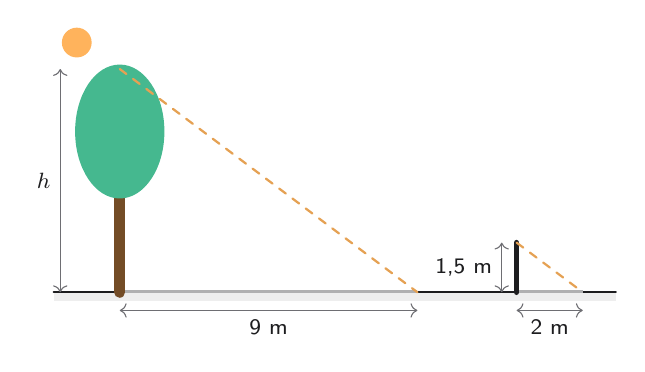
\begin{tikzpicture}[font=\small,x=0.42cm,y=0.42cm,line cap=round,line join=round,step={(1,1)}]
\fill[gris!12] (-2,-0.25) rectangle (15,0);
\draw[tinta,thick] (-2,0)--(15,0);
\fill[tinta!35] (0,-0.03) rectangle (9,0.08);
\draw[brown!60!black,line width=4pt] (0,0)--(0,3.7125000000000004);\fill[menta!80] (0,4.859999999999999) ellipse (1.35 and 2.025);
\draw[narc!90!black,thick,dashed] (0,6.75)--(9,0);
\draw[<->,gris] (-1.8,0)--(-1.8,6.75) node[midway,left,font=\footnotesize,text=tinta] {$h$};
\draw[<->,gris] (0,-0.55)--(9,-0.55) node[midway,below,font=\footnotesize,text=tinta] {9 m};
\fill[tinta!35] (12,-0.03) rectangle (14,0.08);
\draw[tinta,line width=2pt] (12,0)--(12,1.5);
\draw[narc!90!black,thick,dashed] (12,1.5)--(14,0);
\draw[<->,gris] (11.55,0)--(11.55,1.5) node[midway,left,font=\footnotesize,text=tinta] {1,5 m};
\draw[<->,gris] (12,-0.55)--(14,-0.55) node[midway,below,font=\footnotesize,text=tinta] {2 m};
\fill[narc] (-1.3,7.55) circle (0.45);
\end{tikzpicture}
\end{document}
